% =====================================================================
%  Mothbox — Paramétrer sa Mothbox avec un téléphone
%  Compilation : pdfLaTeX ou LuaLaTeX
% =====================================================================
\documentclass[11pt,a4paper,openany]{report}
% =====================================================================
%  Préambule — compatible pdfLaTeX (Overleaf par défaut), XeLaTeX et LuaLaTeX
% =====================================================================
\usepackage{iftex}
\ifPDFTeX
  \usepackage[T1]{fontenc}
  \usepackage[utf8]{inputenc}
\fi
\usepackage{amsmath}
\usepackage[french]{babel}
\usepackage{libertinus}
\usepackage{microtype}

\usepackage[a4paper,top=2.5cm,bottom=2.5cm,left=2.4cm,right=2.4cm,headheight=14pt]{geometry}
\usepackage[table]{xcolor}
\usepackage{graphicx}

\usepackage[locale=FR,per-mode=symbol,group-minimum-digits=4]{siunitx}
\sisetup{range-phrase={\,\text{à}\,},list-final-separator={ et },inter-unit-product=\ensuremath{\cdot}}

\usepackage{booktabs}
\usepackage{tabularx}
\usepackage{longtable}
\usepackage{multirow}
\usepackage{array}
\usepackage{makecell}
\usepackage{caption}
\usepackage{subcaption}
\usepackage{float}
\usepackage{enumitem}
\usepackage{pdflscape}
\usepackage{eso-pic}

\usepackage{pifont}
\usepackage{tikz}
\usetikzlibrary{babel}
\usetikzlibrary{arrows.meta,positioning,fit,calc}

\usepackage[most]{tcolorbox}
\usepackage{listings}
\usepackage{fancyhdr}
\usepackage{titlesec}
\usepackage[hidelinks]{hyperref}
\usepackage[french,nameinlink]{cleveref}

% ---------------------------------------------------------------------
%  Couleurs
% ---------------------------------------------------------------------
\definecolor{pslbleu}{HTML}{1F4E8C}
\definecolor{pslbleuclair}{HTML}{E8EEF7}
\definecolor{pslorange}{HTML}{E8781A}
\definecolor{pslorangeclair}{HTML}{FDF0E4}
\definecolor{pslvert}{HTML}{2E7D4F}
\definecolor{pslvertclair}{HTML}{E7F3EC}
\definecolor{pslrouge}{HTML}{B3261E}
\definecolor{pslrougeclair}{HTML}{FBEAE9}
\definecolor{pslgris}{HTML}{5F6368}

\hypersetup{colorlinks=true,linkcolor=pslbleu,urlcolor=pslbleu,citecolor=pslbleu,
  pdftitle={OpenFlexure USB — Microscope en périphérique USB},
  pdfauthor={Tom Penfornis},pdfsubject={Liaison USB gadget et mise à l'heure}}

% ---------------------------------------------------------------------
%  Titres et en-têtes
% ---------------------------------------------------------------------
\titleformat{\chapter}[display]
  {\normalfont\sffamily\color{pslbleu}}
  {\large\MakeUppercase{\chaptertitlename}~\thechapter}
  {4pt}
  {\Huge\bfseries}
  [\vspace{4pt}{\color{pslorange}\titlerule[1.5pt]}]
\titlespacing*{\chapter}{0pt}{-10pt}{24pt}
\titleformat{\section}{\normalfont\sffamily\Large\bfseries\color{pslbleu}}{\thesection}{0.8em}{}
\titleformat{\subsection}{\normalfont\sffamily\large\bfseries\color{pslbleu!85!black}}{\thesubsection}{0.8em}{}
\titleformat{\subsubsection}{\normalfont\sffamily\normalsize\bfseries}{\thesubsubsection}{0.8em}{}

\pagestyle{fancy}
\fancyhf{}
\fancyhead[L]{\small\sffamily\color{pslgris}OpenFlexure USB — Rapport technique}
\fancyhead[R]{\small\sffamily\color{pslgris}\nouppercase{\leftmark}}
\fancyfoot[C]{\small\sffamily\thepage}
\renewcommand{\headrulewidth}{0.4pt}
\renewcommand{\headrule}{{\color{pslbleu!40}\hrule height\headrulewidth width\headwidth\vskip-\headrulewidth}}
\fancypagestyle{plain}{\fancyhf{}\fancyfoot[C]{\small\sffamily\thepage}\renewcommand{\headrulewidth}{0pt}}

\setcounter{tocdepth}{2}
\setcounter{secnumdepth}{3}
\setlength{\parskip}{0.35em}
\setlist{itemsep=2pt,topsep=4pt}

\captionsetup{font=small,labelfont={bf,sf,color=pslbleu},format=hang,margin=10pt}
\captionsetup[table]{position=top}
\renewcommand{\arraystretch}{1.18}
\newcolumntype{L}{>{\raggedright\arraybackslash}X}
\newcolumntype{C}{>{\centering\arraybackslash}X}

% ---------------------------------------------------------------------
%  Encadrés
% ---------------------------------------------------------------------
\newtcolorbox{synthese}[1][Synthèse]{enhanced,breakable,colback=pslbleuclair,colframe=pslbleu,
  fonttitle=\sffamily\bfseries,title={#1},arc=2pt,boxrule=0.6pt,left=6pt,right=6pt}
\newtcolorbox{choix}[1][Choix retenu]{enhanced,breakable,colback=pslvertclair,colframe=pslvert,
  fonttitle=\sffamily\bfseries,title={#1},arc=2pt,boxrule=0.6pt,left=6pt,right=6pt}
\newtcolorbox{attention}[1][Point de vigilance]{enhanced,breakable,colback=pslrougeclair,colframe=pslrouge,
  fonttitle=\sffamily\bfseries,title={#1},arc=2pt,boxrule=0.6pt,left=6pt,right=6pt}
\newtcolorbox{calcul}[1][Calcul]{enhanced,breakable,colback=white,colframe=pslorange,
  fonttitle=\sffamily\bfseries,coltitle=black,colbacktitle=pslorangeclair,title={#1},arc=2pt,boxrule=0.6pt,left=6pt,right=6pt}

% ---------------------------------------------------------------------
%  Code
% ---------------------------------------------------------------------
\lstdefinestyle{psl}{basicstyle=\ttfamily\footnotesize,keywordstyle=\color{pslbleu},
  commentstyle=\color{pslgris}\itshape,stringstyle=\color{pslorange!80!black},numbers=left,
  numberstyle=\tiny\color{pslgris},frame=single,rulecolor=\color{pslbleu!30},backgroundcolor=\color{pslbleuclair!40},
  breaklines=true,columns=fullflexible,keepspaces=true,showstringspaces=false,
  literate={é}{{\'e}}1 {è}{{\`e}}1 {à}{{\`a}}1 {ç}{{\c{c}}}1 {ê}{{\^e}}1 {É}{{\'E}}1 {ô}{{\^o}}1 {î}{{\^i}}1 {û}{{\^u}}1 {ù}{{\`u}}1 {Ø}{{\O}}1 {×}{{$\times$}}1 {â}{{\^a}}1 {⇄}{{$\leftrightarrows$}}1 {→}{{$\rightarrow$}}1 {«}{{\guillemotleft}}1 {»}{{\guillemotright}}1 {À}{{\`A}}1}
\lstset{style=psl}

% ---------------------------------------------------------------------
%  Raccourcis
% ---------------------------------------------------------------------
\newcommand{\comp}[1]{\textsf{#1}}
\newcommand{\fichier}[1]{{\small\nolinkurl{#1}}}

% Pas de citation (lien dans un lien) dans les listes des figures et des tableaux
\let\listoffiguresorig\listoffigures
\let\listoftablesorig\listoftables
\renewcommand{\listoffigures}{\begingroup\renewcommand{\cite}[2][]{}\listoffiguresorig\endgroup}
\renewcommand{\listoftables}{\begingroup\renewcommand{\cite}[2][]{}\listoftablesorig\endgroup}
\crefname{lstlisting}{listing}{listings}
\Crefname{lstlisting}{Listing}{Listings}


\hypersetup{pdftitle={Paramétrer sa Mothbox avec un téléphone},
  pdfsubject={Guide d'utilisation de l'interface de terrain Mothbox}}
\fancyhead[L]{\small\sffamily\color{pslgris}Mothbox — Guide de terrain}
\graphicspath{{annotees/}}
\newcommand{\sw}[1]{\textsf{\bfseries #1}}
\newcommand{\on}{\textcolor{pslvert}{\textsf{\bfseries ON}}}
\newcommand{\off}{\textcolor{pslrouge}{\textsf{\bfseries OFF}}}
\newcommand{\pasc}[2]{\tikz[baseline=(n.base)]\node[circle,fill=#1,text=white,font=\sffamily\bfseries\footnotesize,inner sep=1.5pt,minimum size=1.2em](n){#2};}
\newcommand{\pas}[1]{\pasc{pslrouge}{#1}}
\newtcolorbox{astuce}[1][Bon réflexe]{enhanced,breakable,colback=pslvertclair,colframe=pslvert,
  fonttitle=\sffamily\bfseries,title={#1},arc=2pt,boxrule=0.6pt,left=6pt,right=6pt}

\begin{document}

\pagenumbering{Alph}
\begin{titlepage}
\begin{tikzpicture}[remember picture,overlay]
  \fill[pslvert] (current page.north west) rectangle ([yshift=-8.2cm]current page.north east);
  \fill[pslorange] ([yshift=-8.2cm]current page.north west) rectangle ([yshift=-8.5cm]current page.north east);
  \node[anchor=north west,text=white!85!pslvert,font=\sffamily\small,inner sep=0pt] at ([xshift=2.4cm,yshift=-1.7cm]current page.north west) {Mothbox Pro — PSL3D};
  \node[anchor=north west,text=white,font=\sffamily\bfseries\fontsize{30}{36}\selectfont,inner sep=0pt,text width=16.5cm] at ([xshift=2.4cm,yshift=-2.6cm]current page.north west) {Paramétrer sa Mothbox avec un téléphone};
  \node[anchor=north west,text=white!90!pslvert,font=\sffamily\Large,inner sep=0pt,text width=16cm] at ([xshift=2.4cm,yshift=-6.25cm]current page.north west) {Deux switches, un wifi, une page web};
\end{tikzpicture}

\vspace*{8.2cm}
\begin{center}
\begin{tikzpicture}[font=\sffamily\small,
  boite/.style={draw=pslvert,fill=pslvertclair,rounded corners=3pt,minimum height=1.5cm,align=center,line width=0.8pt},
  lien/.style={line width=1.4pt,pslorange}]
  \node[boite,minimum width=3.8cm] (tel) {\textbf{Votre téléphone}\\navigateur web};
  \node[boite,minimum width=3.8cm,right=4.2cm of tel] (mb) {\textbf{Mothbox}\\switch \sw{DEBUG} sur ON};
  \draw[lien,{Latex}-{Latex}] (tel) -- node[above,text=black]{wifi \texttt{Mothbox-…}} node[below,text=black,font=\sffamily\footnotesize]{sans Internet} (mb);
\end{tikzpicture}
\end{center}
\vfill
{\sffamily
\begin{tabularx}{\textwidth}{@{}lL@{}}
\toprule
\textbf{Pour qui} & Toute personne qui installe une Mothbox sur le terrain, même sans aucune connaissance en informatique \\
\textbf{Il faut} & Une Mothbox avec l'image \texttt{5.2.1-webui}, un téléphone (iPhone ou Android) \\
\textbf{Auteur} & Tom Penfornis \\
\textbf{Version} & 1.0 --- 26 novembre 2026 \\
\bottomrule
\end{tabularx}}
\end{titlepage}

\pagenumbering{roman}
\chapter*{L'essentiel en une page}
\addcontentsline{toc}{chapter}{L'essentiel en une page}

\begin{synthese}[En bref]
Avant, pour régler une Mothbox, il fallait un ordinateur, le logiciel VNC, un identifiant et savoir quel fichier modifier.
Désormais, \textbf{un téléphone suffit} : la Mothbox crée son propre wifi et affiche une page qui guide pas à pas.
\end{synthese}

\begin{enumerate}[label=\protect\pas{\arabic*},leftmargin=2.2em,itemsep=6pt]
  \item Mettre les switches \sw{Active} et \sw{DEBUG} sur \on{}, puis brancher la batterie.
  \item Attendre 2 à 3 minutes, puis connecter le téléphone au wifi \texttt{Mothbox-…} (mot de passe \texttt{lunaluna}). La page s'ouvre toute seule.
  \item Suivre les 4 étapes de la page : \emph{Heure}, \emph{Planning}, \emph{Tester}, \emph{Terminer}.
  \item Remettre \sw{DEBUG} sur \off{} (laisser \sw{Active} sur \on{}) et appuyer sur \emph{Redémarrer maintenant}. La Mothbox est en service.
\end{enumerate}

\begin{attention}[Lire un switch]
Un switch est sur \on{} quand son levier est poussé \textbf{du côté de l'inscription \og ON \fg{} imprimée sur le boîtier noir}. Sur la carte Mothbox, cette inscription est à l'envers et se lit \og NO \fg{} : c'est le côté \textbf{bas} sur toutes les photos de ce guide.
\end{attention}

\begin{astuce}[Les trois switches à connaître]
\sw{Active} : la Mothbox travaille (\on) ou reste éteinte (\off). \quad
\sw{DEBUG} : mode réglage avec wifi et page web. \quad
\sw{U1} : planning réglé par les switches de la carte au lieu de la page (facultatif).
\end{astuce}

\tableofcontents

\clearpage
\pagenumbering{arabic}

% ---------------------------------------------------------------------
\chapter{Repérer les switches}
% ---------------------------------------------------------------------

La carte Mothbox porte quatre rangées de petits switches. Pour l'utilisation courante, seuls \textbf{deux} comptent : \sw{Active} et \sw{DEBUG}.

\begin{figure}[H]
\centering
\begin{minipage}[c]{0.42\textwidth}
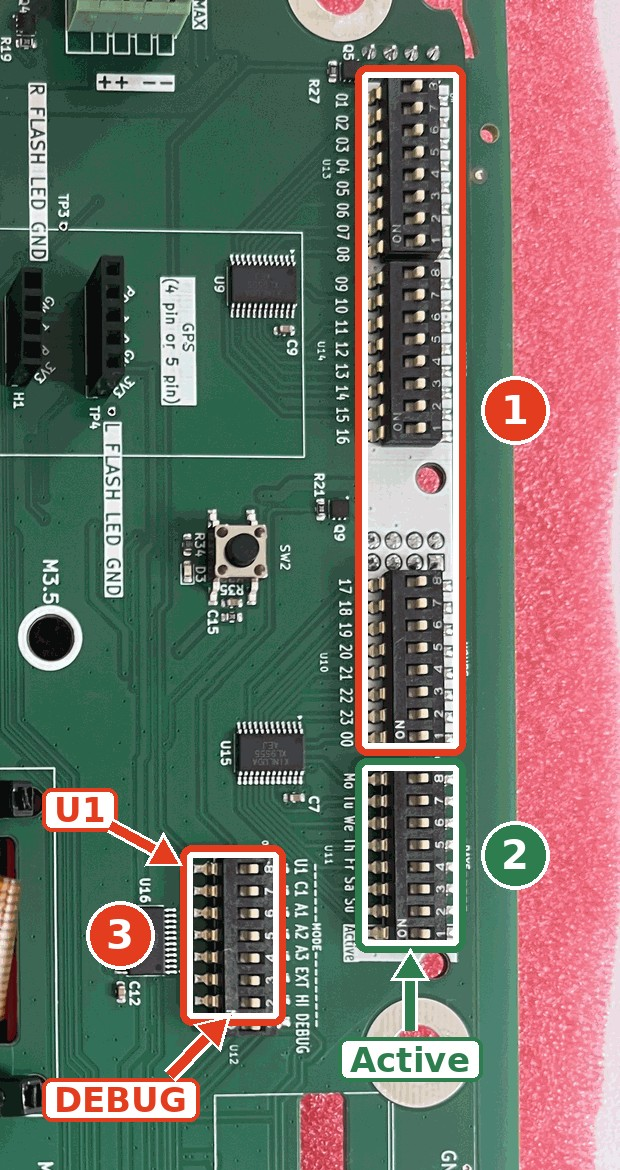
\includegraphics[width=\linewidth]{carte_reperes.jpg}
\end{minipage}\hfill
\begin{minipage}[c]{0.53\textwidth}
\begin{description}[leftmargin=0pt,itemsep=8pt]
  \item[\pas{1} Heures (01 à 00)] 24 switches, un par heure. Ils ne servent qu'en mode manuel (\cref{chmanuel}).
  \item[\pas{2} Jours + Active] 7 switches de jours (Mo à Su), utilisés en mode manuel, et le switch \sw{Active}, \textbf{le plus important} : sans lui, la Mothbox ne fait rien.
  \item[\pas{3} Mode] \sw{U1}, \sw{C1}, \sw{A1}–\sw{A3}, \sw{EXT}, \sw{HI} et \sw{DEBUG}. Leur rôle est détaillé juste en dessous.
\end{description}
\end{minipage}
\caption{Les trois zones de switches de la carte Mothbox v5.0.5.}
\end{figure}

\section*{À quoi servent les switches de la rangée MODE ?}
\addcontentsline{toc}{section}{À quoi servent les switches de la rangée MODE ?}

\begin{figure}[H]
\centering
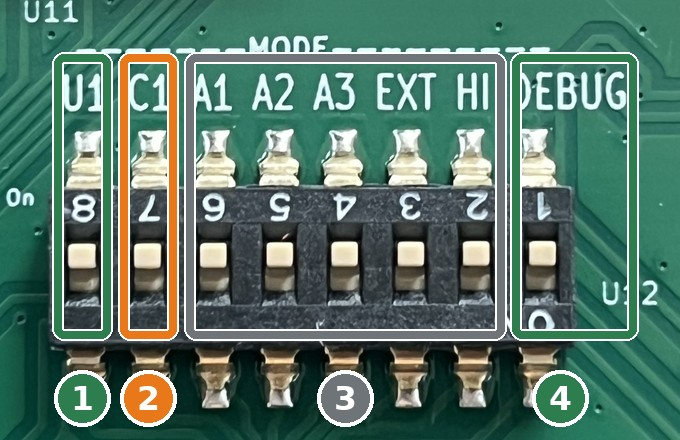
\includegraphics[width=0.62\textwidth]{rangee_mode.jpg}
\caption{La rangée MODE. En vert : les switches utiles au quotidien ; en orange : un test d'atelier ; en gris : des switches réservés, sans effet aujourd'hui.}
\end{figure}

\begin{table}[H]
\centering\sffamily\small
\caption{Rôle de chaque switch de la rangée MODE (logiciel Mothbox 5.2.1).}
\begin{tabularx}{\textwidth}{@{}c>{\raggedright\arraybackslash}p{2.1cm}L@{}}
\toprule
 & Switch & Rôle \\
\midrule
\pasc{pslvert}{1} & \sw{U1} & \textbf{Mode manuel.} Sur \on, le planning est réglé par les switches d'heures et de jours de la carte, et plus par la page (\cref{chmanuel}). \\
\pasc{pslorange}{2} & \sw{C1} & \textbf{Test des lumières} (mode \og fête \fg{}). Seulement avec \sw{DEBUG} sur \on : toutes les voies d'éclairage (voies 1, 2, 3, sortie externe) et le flash clignotent à tour de rôle, en boucle, pour vérifier d'un coup d'œil que chaque voie est bien câblée. Ne s'arrête qu'au redémarrage. \textbf{Laissez-le sur \off{} quand vous utilisez la page}, sinon il brouille les tests de l'étape 3. \\
\pasc{pslgris}{3} & \sw{A1} \sw{A2} \sw{A3} & \textbf{Réservés.} Prévus pour choisir individuellement les voies d'attraction 1, 2 et 3. Pas encore lus par le logiciel : toutes les voies s'allument ensemble quelle que soit leur position. \\
 & \sw{EXT} & \textbf{Réservé.} Prévu pour la sortie d'attraction externe (bornier \og Ext \fg{}). Pas encore lu : cette sortie s'allume avec les autres. \\
 & \sw{HI} & \textbf{Réservé.} Prévu pour un fonctionnement sur alimentation secteur (wifi maintenu, envoi des photos). Aujourd'hui, la Mothbox se comporte exactement comme en service normal. \\
\pasc{pslvert}{4} & \sw{DEBUG} & \textbf{Mode réglage.} Wifi, page web, aucune mise en veille ni capture automatique (\cref{chpas}). \\
\bottomrule
\end{tabularx}
\end{table}

\begin{astuce}[En pratique]
Laissez \sw{C1}, \sw{A1}, \sw{A2}, \sw{A3}, \sw{EXT} et \sw{HI} sur \off. Seuls \sw{Active}, \sw{DEBUG} et, si besoin, \sw{U1} servent au quotidien.
\end{astuce}

% ---------------------------------------------------------------------
\chapter{Les quatre positions à connaître}
% ---------------------------------------------------------------------

Les switches ne sont lus qu'\textbf{au démarrage} de la Mothbox. Après avoir changé un switch, il faut donc redémarrer (débrancher puis rebrancher la batterie, ou utiliser le bouton de la page).

\begin{table}[H]
\centering\sffamily\small
\caption{Ce que fait la Mothbox selon la position de \sw{Active} et \sw{DEBUG}.}
\begin{tabularx}{\textwidth}{@{}llL@{}}
\toprule
\sw{Active} & \sw{DEBUG} & Ce qui se passe \\
\midrule
\off & \off & \textbf{Rangement, transport, charge.} La Mothbox s'éteint aussitôt qu'elle se réveille. \\
\on & \on & \textbf{Réglage.} Elle reste allumée, crée son wifi et affiche la page. Aucune capture. \\
\on & \off & \textbf{En service.} Elle dort et se réveille aux heures prévues pour attirer et photographier. \\
\off & \on & \textbf{Erreur fréquente.} \sw{Active} prime : la Mothbox s'éteint, pas de wifi ni de page. \\
\bottomrule
\end{tabularx}
\end{table}

\begin{figure}[H]
\centering
\begin{subfigure}[t]{0.34\textwidth}\centering
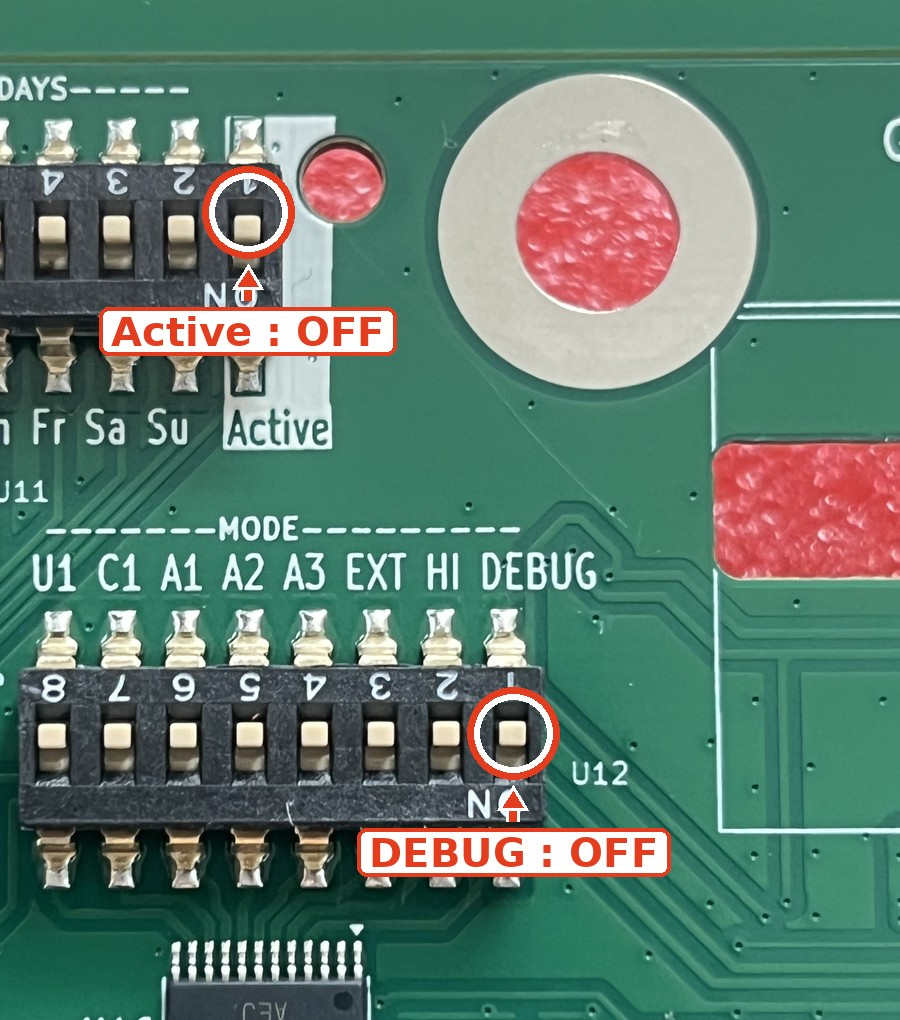
\includegraphics[width=\linewidth]{pos_tout_off.jpg}
\caption{Rangement : tout sur \off.}
\end{subfigure}\hspace{0.04\textwidth}
\begin{subfigure}[t]{0.34\textwidth}\centering
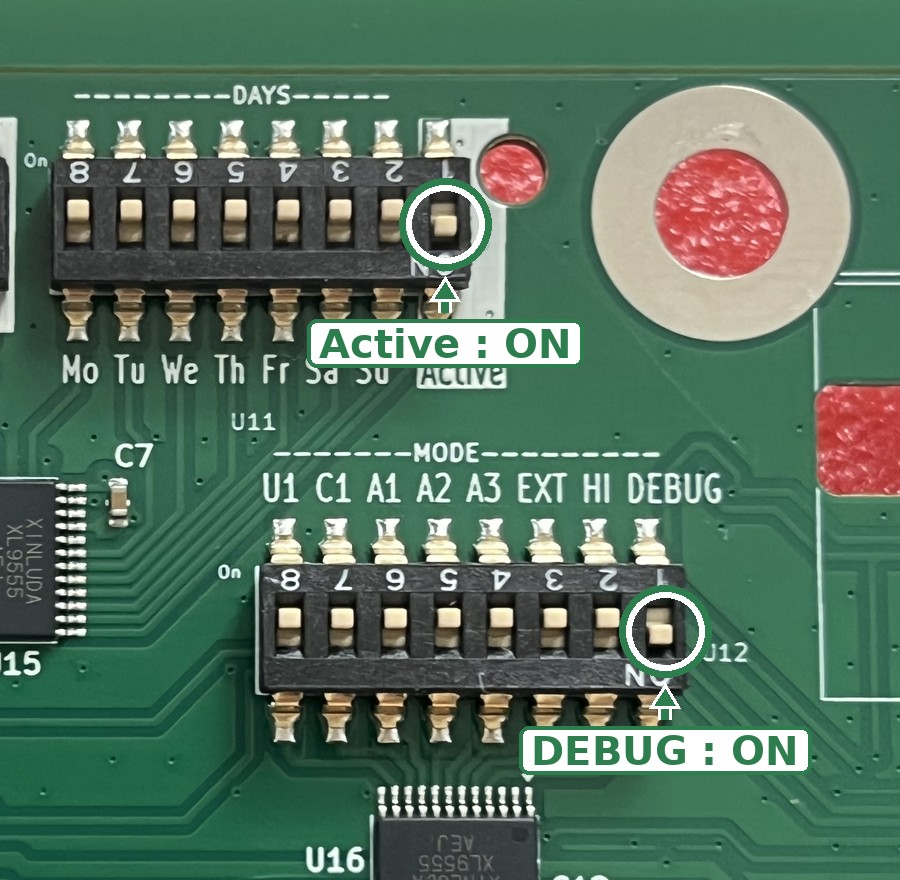
\includegraphics[width=\linewidth]{pos_active_debug.jpg}
\caption{Réglage avec le téléphone : \sw{Active} et \sw{DEBUG} sur \on.}
\end{subfigure}

\vspace{8pt}
\begin{subfigure}[t]{0.34\textwidth}\centering
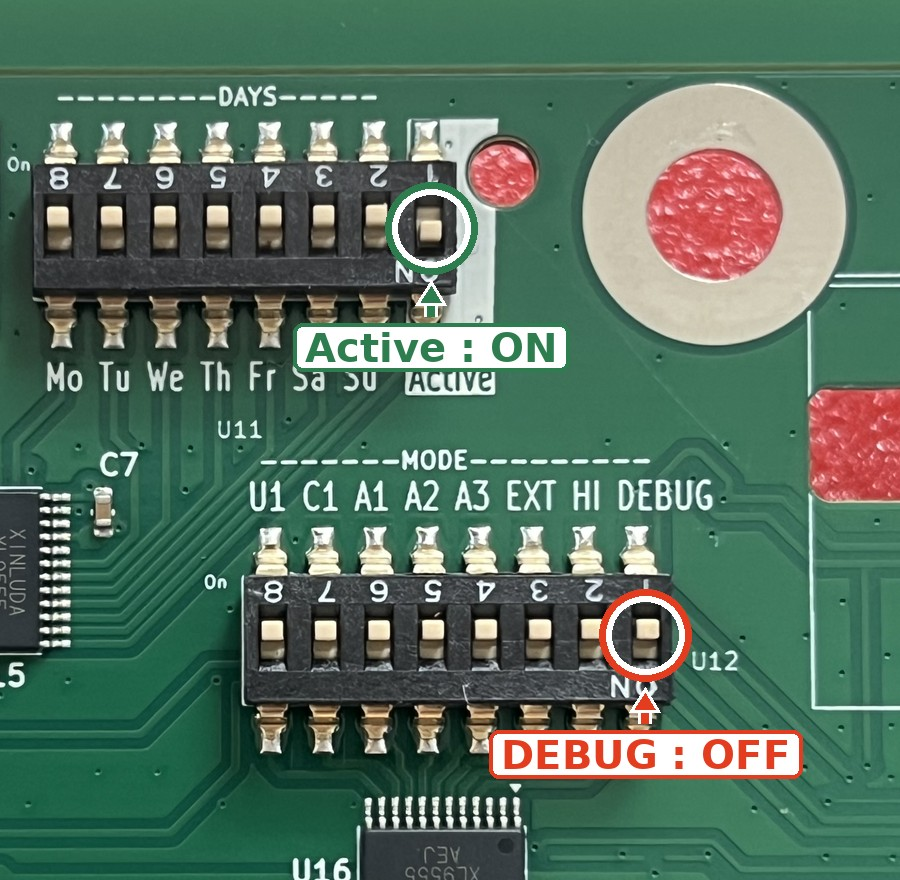
\includegraphics[width=\linewidth]{pos_active_seul.jpg}
\caption{En service : \sw{Active} sur \on, \sw{DEBUG} sur \off.}
\end{subfigure}\hspace{0.04\textwidth}
\begin{subfigure}[t]{0.34\textwidth}\centering
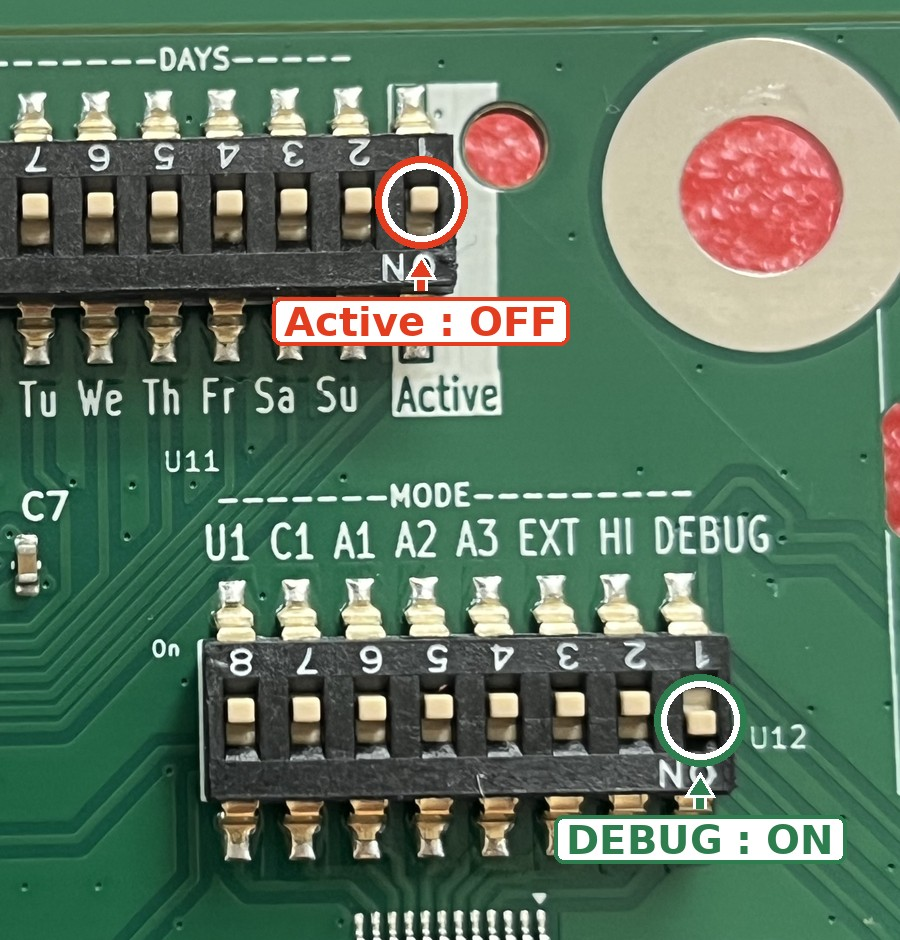
\includegraphics[width=\linewidth]{pos_debug_sans_active.jpg}
\caption{À éviter : \sw{DEBUG} sur \on{} mais \sw{Active} sur \off.}
\end{subfigure}
\caption{Les quatre positions, photographiées sur la carte. Les anneaux verts montrent un switch sur \on, les rouges un switch sur \off.}
\end{figure}

% ---------------------------------------------------------------------
\chapter{Régler la Mothbox pas à pas}\label{chpas}
% ---------------------------------------------------------------------

\section{Se connecter}

\begin{enumerate}[label=\protect\pas{\arabic*},leftmargin=2.2em,itemsep=5pt]
  \item Mettre \sw{Active} et \sw{DEBUG} sur \on, puis brancher la batterie.
  \item Attendre \textbf{2 à 3 minutes} : la Mothbox démarre puis crée son wifi.
  \item Dans les réglages wifi du téléphone, choisir le réseau \texttt{Mothbox-} suivi du nom de la boîte (par exemple \texttt{Mothbox-adultoAngu}). Mot de passe : \texttt{lunaluna}.
  \item La page s'ouvre toute seule. Si ce n'est pas le cas, ouvrir le navigateur et taper \texttt{192.168.50.5}.
\end{enumerate}

\begin{astuce}[Le téléphone dit \og pas d'accès Internet \fg{}]
C'est normal : la Mothbox n'est pas reliée à Internet. Choisissez \emph{Rester connecté} ou \emph{Utiliser ce réseau tel quel}.
\end{astuce}

La page est en français ou en anglais selon la langue du téléphone ; le bouton \textsf{EN}/\textsf{FR} en haut à droite permet de changer. Les étapes se suivent avec le bouton \emph{Étape suivante}, mais on peut aussi toucher directement un numéro en haut.

\section{Étape 1 — Heure et lieu}

\begin{minipage}[t]{0.36\textwidth}
\vspace{0pt}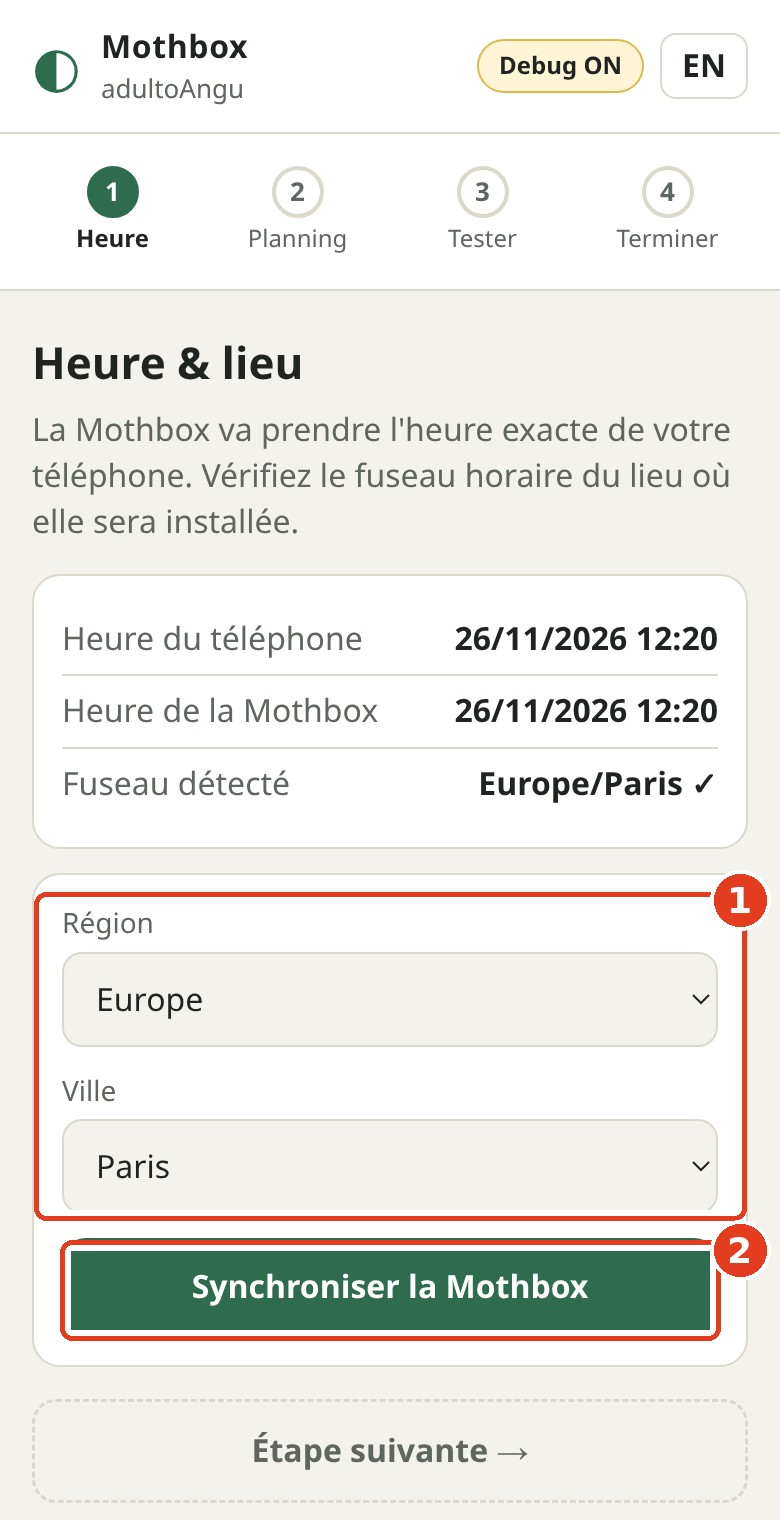
\includegraphics[width=\linewidth]{ecran_etape1.jpg}
\end{minipage}\hfill
\begin{minipage}[t]{0.6\textwidth}
\vspace{0pt}
La Mothbox n'a pas d'accès à Internet pour se mettre à l'heure : elle prend celle du téléphone.
\begin{description}[leftmargin=0pt,itemsep=6pt]
  \item[\pas{1} Fuseau horaire] Il est détecté à partir du téléphone. S'il ne correspond pas au lieu d'installation (téléphone resté à l'heure d'un autre pays), choisissez la région puis la ville.
  \item[\pas{2} Synchroniser la Mothbox] Un message confirme la mise à l'heure et indique l'écart corrigé.
\end{description}
Si le fuseau n'a pas pu être détecté, le bouton reste grisé tant qu'aucune ville n'est choisie.
\end{minipage}

\section{Étape 2 — Planning des captures}

\begin{minipage}[t]{0.36\textwidth}
\vspace{0pt}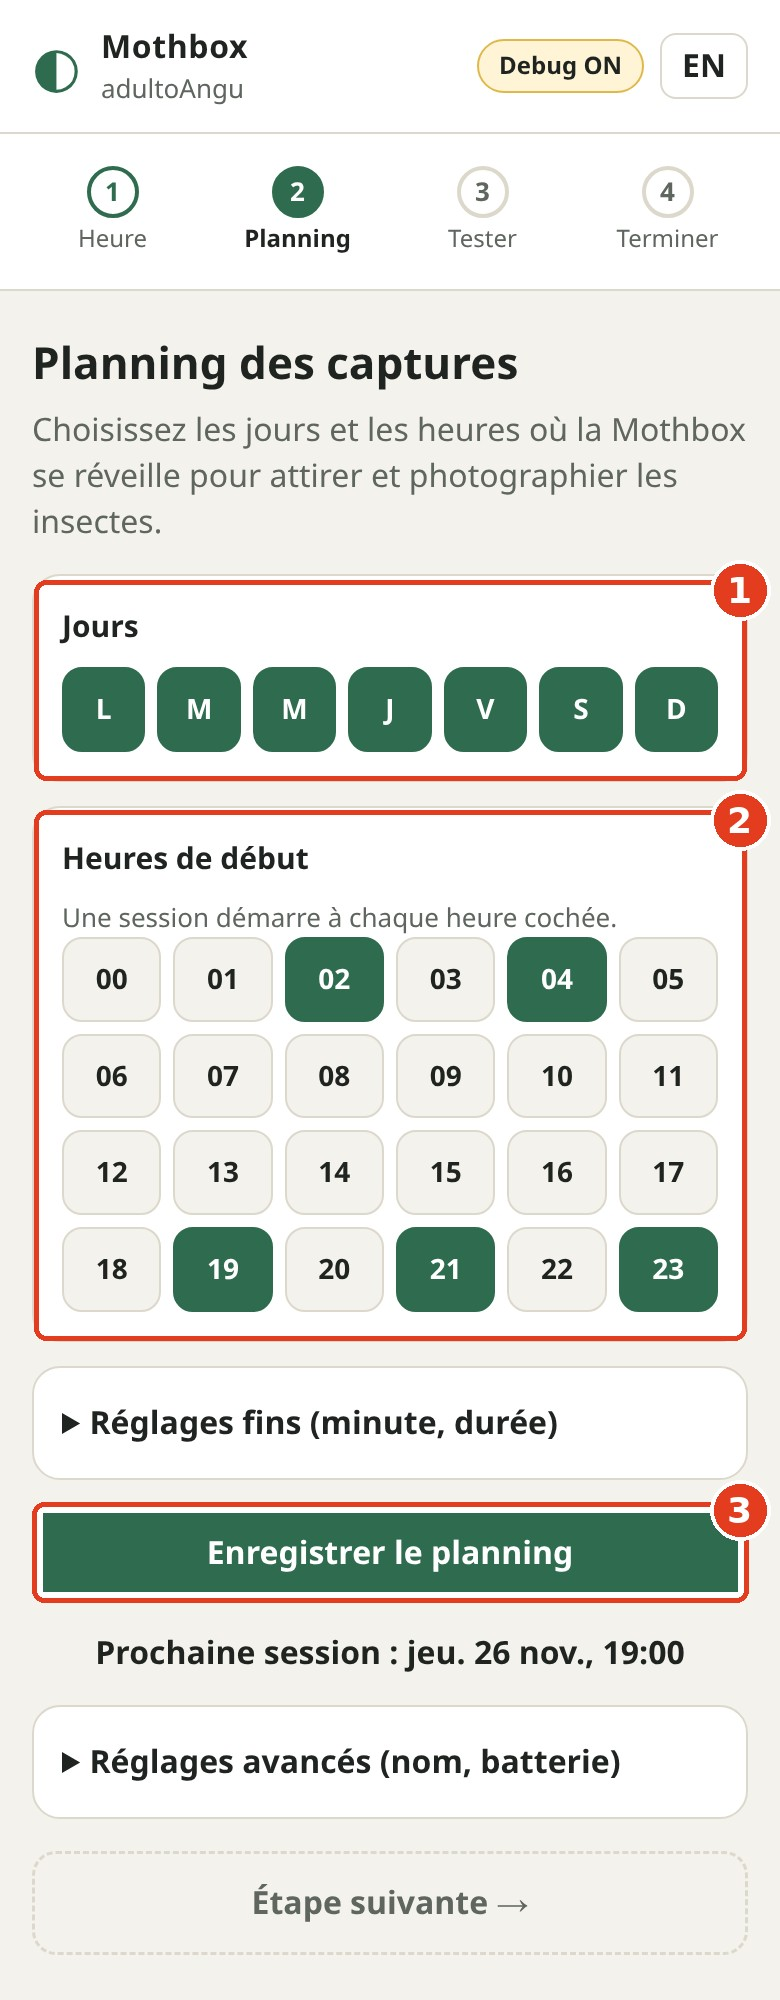
\includegraphics[width=\linewidth]{ecran_etape2.jpg}
\end{minipage}\hfill
\begin{minipage}[t]{0.6\textwidth}
\vspace{0pt}
Le planning dit quand la Mothbox se réveille pour allumer sa lumière et photographier.
\begin{description}[leftmargin=0pt,itemsep=6pt]
  \item[\pas{1} Jours] Touchez un jour pour l'activer (vert) ou le désactiver.
  \item[\pas{2} Heures de début] Une session démarre à chaque heure cochée.
  \item[\pas{3} Enregistrer le planning] La ligne \emph{Prochaine session} se met à jour.
\end{description}
\textbf{Réglages fins} : minute de départ (par exemple 19\,h\,15) et durée de chaque session (59 minutes par défaut).

\textbf{Réglages avancés} : nom de la Mothbox (il donne aussi son nom au wifi, après redémarrage) et caractéristiques de la batterie, pour un pourcentage juste.
\end{minipage}

\section{Étape 3 — Tester}

\begin{minipage}[t]{0.36\textwidth}
\vspace{0pt}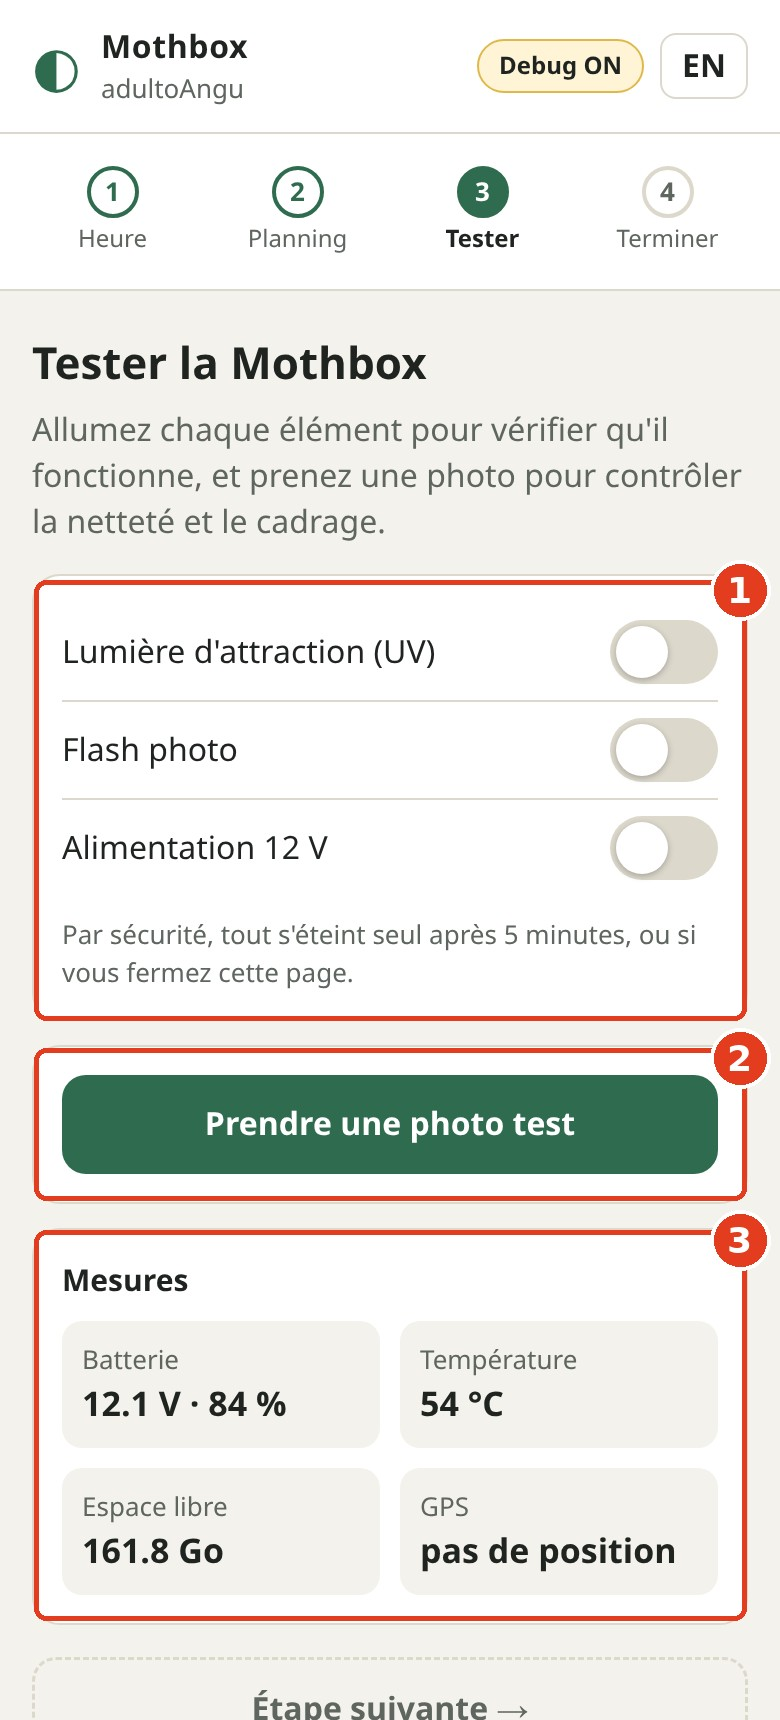
\includegraphics[width=\linewidth]{ecran_etape3.jpg}
\end{minipage}\hfill
\begin{minipage}[t]{0.6\textwidth}
\vspace{0pt}
\begin{description}[leftmargin=0pt,itemsep=6pt]
  \item[\pas{1} Interrupteurs] Allumez la lumière d'attraction (UV), le flash et l'alimentation 12\,V pour vérifier qu'ils fonctionnent. Un compte à rebours s'affiche.
  \item[\pas{2} Photo test] La photo s'affiche sur le téléphone. Le drap doit être net et remplir l'image : c'est le moment d'ajuster la position de la Mothbox.
  \item[\pas{3} Mesures] Tension et charge de la batterie, température, espace libre sur la carte SD et position GPS si un module est branché.
\end{description}
\begin{astuce}[Sécurité]
Tout s'éteint seul au bout de 5 minutes, ou 30 secondes après la fermeture de la page. Impossible de vider la batterie en oubliant la lumière allumée.
\end{astuce}
\end{minipage}

\section{Étape 4 — Mettre en service}

\begin{minipage}[t]{0.36\textwidth}
\vspace{0pt}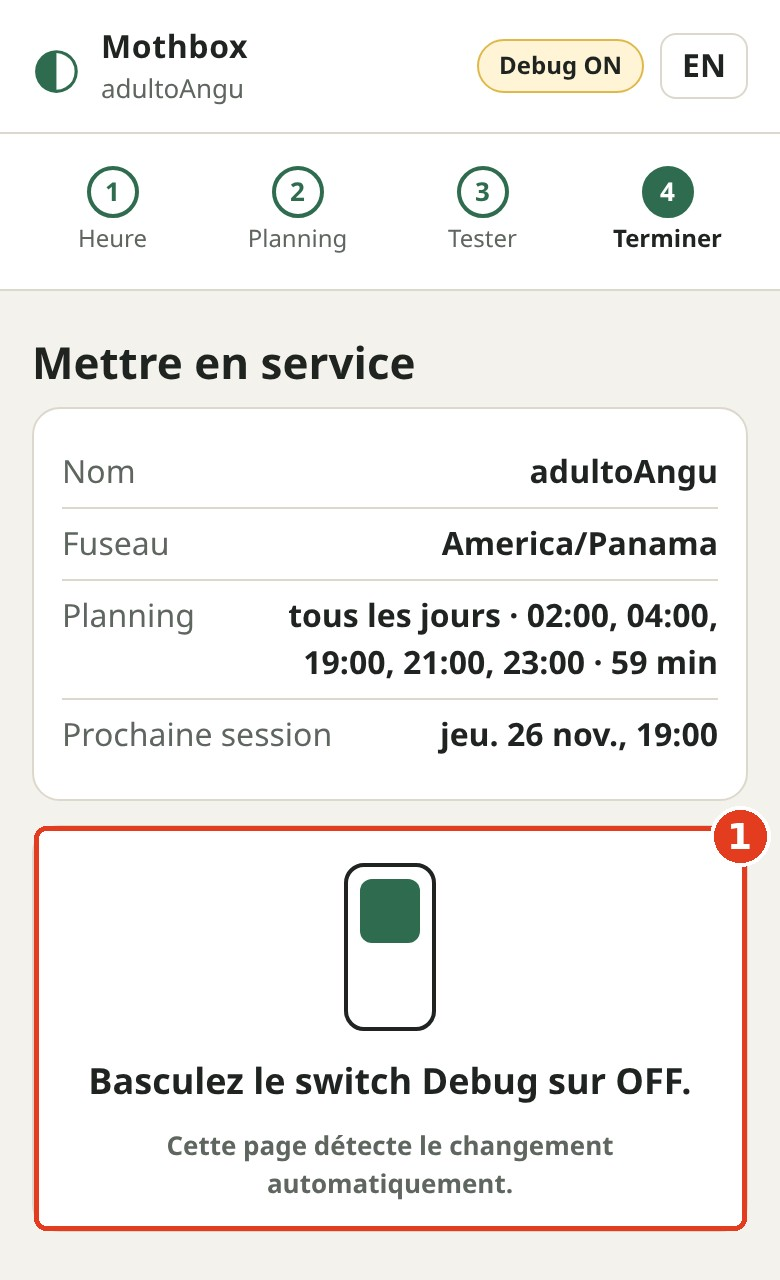
\includegraphics[width=\linewidth]{ecran_etape4.jpg}

\vspace{6pt}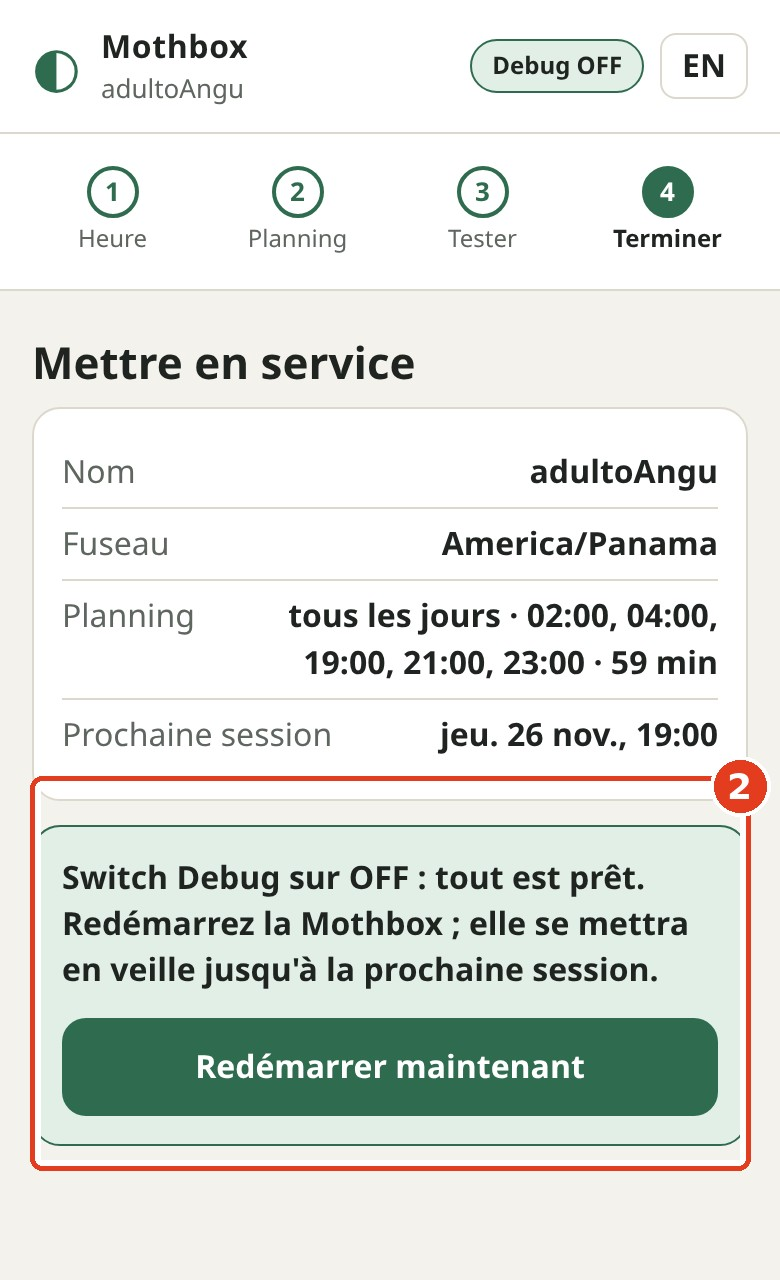
\includegraphics[width=\linewidth]{ecran_etape4_pret.jpg}
\end{minipage}\hfill
\begin{minipage}[t]{0.6\textwidth}
\vspace{0pt}
Un récapitulatif rappelle le nom, le fuseau, le planning et la prochaine session.
\begin{description}[leftmargin=0pt,itemsep=6pt]
  \item[\pas{1} Basculer DEBUG sur OFF] Directement sur la carte, sans débrancher. \textbf{Laissez Active sur ON.} La page détecte le changement en quelques secondes.
  \item[\pas{2} Redémarrer maintenant] La Mothbox redémarre, coupe son wifi et se met en veille jusqu'à la prochaine session. Vous pouvez fermer la page.
\end{description}
\begin{attention}[Si la page affiche \og le switch Active est sur OFF \fg{}]
Remettez \sw{Active} sur \on{} : dans cette position la Mothbox s'éteindrait à chaque réveil sans prendre une seule photo. Le bouton de redémarrage n'apparaît pas tant que c'est le cas.
\end{attention}
\end{minipage}

% ---------------------------------------------------------------------
\chapter{Mode manuel par les switches}\label{chmanuel}
% ---------------------------------------------------------------------

Sans téléphone, on peut régler le planning directement sur la carte.

\begin{enumerate}[label=\protect\pas{\arabic*},leftmargin=2.2em,itemsep=5pt]
  \item Mettre \sw{U1} sur \on.
  \item Mettre sur \on{} les switches des \textbf{heures} de départ voulues (01 à 00) et des \textbf{jours} (Mo à Su).
  \item Redémarrer la Mothbox.
\end{enumerate}

\begin{minipage}[t]{0.36\textwidth}
\vspace{0pt}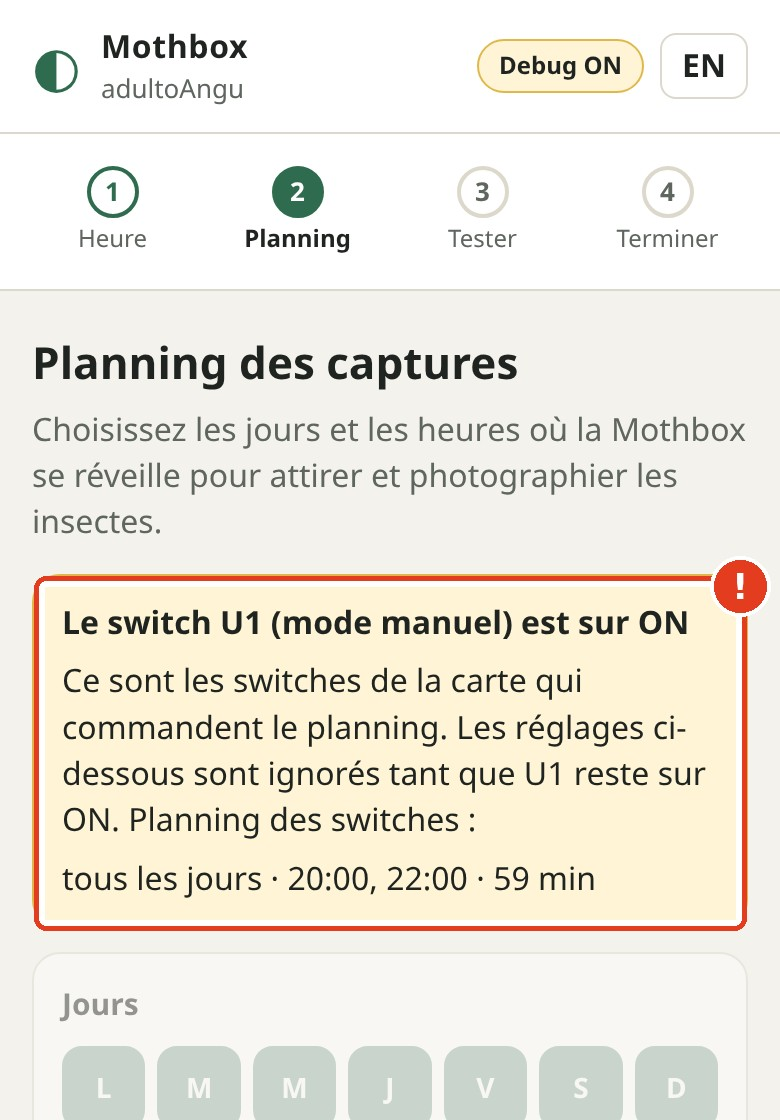
\includegraphics[width=\linewidth]{ecran_etape2_u1.jpg}
\end{minipage}\hfill
\begin{minipage}[t]{0.6\textwidth}
\vspace{0pt}
Tant que \sw{U1} est sur \on, \textbf{les switches de la carte priment} sur la page. La page le signale par un bandeau jaune, affiche le planning lu sur les switches et grise ses propres réglages.

En mode manuel, chaque session démarre à l'heure pile et dure 59 minutes. Pour une autre minute de départ ou une autre durée, utilisez la page (\sw{U1} sur \off).

Si aucun switch d'heure n'est sur \on, la Mothbox applique par défaut 19\,h, 21\,h, 23\,h, 2\,h et 4\,h ; si aucun jour n'est sur \on, elle travaille tous les jours.
\end{minipage}

% ---------------------------------------------------------------------
\chapter{En cas de problème}
% ---------------------------------------------------------------------

\begin{table}[H]
\centering\sffamily\small
\caption{Problèmes courants.}
\begin{tabularx}{\textwidth}{@{}>{\raggedright\arraybackslash}p{5.2cm}L@{}}
\toprule
Ce que vous constatez & Ce qu'il faut essayer \\
\midrule
Aucun wifi \texttt{Mothbox-…} & Attendre 3 minutes. Vérifier que \sw{Active} \textbf{et} \sw{DEBUG} sont sur \on, puis redémarrer. Chercher aussi un réseau nommé \texttt{mothboxwifi}. \\
Connecté, mais la page ne s'ouvre pas & Ouvrir le navigateur et taper \texttt{192.168.50.5}. \\
Le téléphone se déconnecte tout seul & Il cherche Internet : choisir \emph{Rester connecté} ; sur Android, désactiver temporairement les données mobiles. \\
\og La carte n'a pas répondu \fg{} & Vérifier les branchements de la lumière et du flash, puis réessayer. \\
\og La caméra n'a pas répondu \fg{} & Vérifier la nappe de la caméra (connecteur bien enfoncé), puis réessayer. \\
La page attend le switch DEBUG & Vérifier que c'est bien le switch \sw{DEBUG} (le dernier de la rangée MODE) qui a été basculé. \\
Les photos sont prises aux mauvaises heures & Refaire l'étape 1 (fuseau) ; vérifier que \sw{U1} est sur \off{} si le planning a été réglé sur la page. \\
La Mothbox ne prend aucune photo & Vérifier que \sw{Active} est sur \on{} et \sw{DEBUG} sur \off. \\
\bottomrule
\end{tabularx}
\end{table}

% ---------------------------------------------------------------------
\chapter{Pour l'équipe : préparer une carte SD}
% ---------------------------------------------------------------------

L'image \fichier{mothbox_Pro_Pi5_v5.2.1-webui_2026-11-26.zip} contient le système Mothbox 5.2.1 d'origine, complété par la page de réglage. Aucun wifi n'y est enregistré.

\begin{enumerate}[label=\protect\pas{\arabic*},leftmargin=2.2em,itemsep=5pt]
  \item Ouvrir \textbf{Raspberry Pi Imager}, choisir \emph{Raspberry Pi 5}, puis \emph{Utiliser une image personnalisée} et sélectionner le fichier \fichier{.zip}.
  \item Choisir la carte SD (16\,Go minimum) et écrire. Ne pas appliquer de personnalisation de l'OS.
  \item Insérer la carte dans la Mothbox et suivre le \cref{chmanuel} ou le chapitre 3.
\end{enumerate}

Sous Linux, en ligne de commande, après décompression :
\begin{lstlisting}[language=bash,numbers=none]
sudo dd if=mothbox_Pro_Pi5_v5.2.1-webui_2026-11-26.img of=/dev/sdX bs=4M status=progress conv=fsync
\end{lstlisting}
\texttt{/dev/sdX} est la carte SD : vérifiez-le avec \texttt{lsblk}, une erreur efface le mauvais disque.

\end{document}
